\documentclass{standalone}
\usepackage{tikz}
\usetikzlibrary{patterns, positioning}


\begin{document}
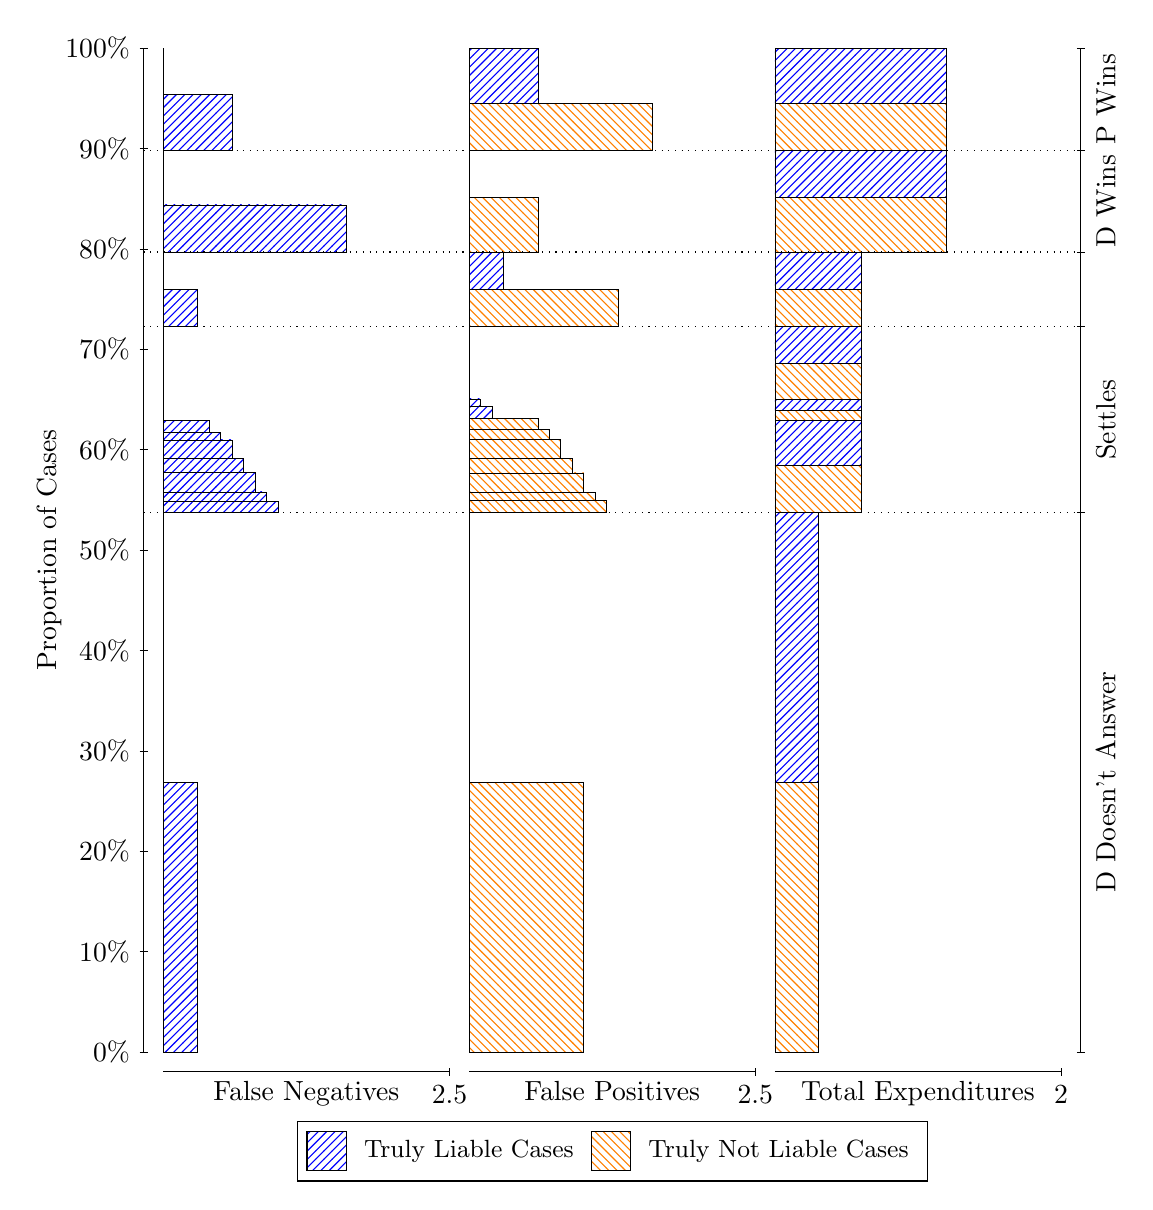
\begin{tikzpicture}
\draw[black, very thin] (1.5,1.75) -- (1.5,14.5);
\node[rotate=90, text=black, anchor=center] at (0.3, 8.125) {Proportion of Cases};
\draw[black, very thin] (1.45,1.75) -- (1.55,1.75);
\node[text=black, anchor=east] at (1.45, 1.75) {0\%};
\draw[black, very thin] (1.45,3.025) -- (1.55,3.025);
\node[text=black, anchor=east] at (1.45, 3.025) {10\%};
\draw[black, very thin] (1.45,4.3) -- (1.55,4.3);
\node[text=black, anchor=east] at (1.45, 4.3) {20\%};
\draw[black, very thin] (1.45,5.575) -- (1.55,5.575);
\node[text=black, anchor=east] at (1.45, 5.575) {30\%};
\draw[black, very thin] (1.45,6.85) -- (1.55,6.85);
\node[text=black, anchor=east] at (1.45, 6.85) {40\%};
\draw[black, very thin] (1.45,8.125) -- (1.55,8.125);
\node[text=black, anchor=east] at (1.45, 8.125) {50\%};
\draw[black, very thin] (1.45,9.4) -- (1.55,9.4);
\node[text=black, anchor=east] at (1.45, 9.4) {60\%};
\draw[black, very thin] (1.45,10.675) -- (1.55,10.675);
\node[text=black, anchor=east] at (1.45, 10.675) {70\%};
\draw[black, very thin] (1.45,11.95) -- (1.55,11.95);
\node[text=black, anchor=east] at (1.45, 11.95) {80\%};
\draw[black, very thin] (1.45,13.225) -- (1.55,13.225);
\node[text=black, anchor=east] at (1.45, 13.225) {90\%};
\draw[black, very thin] (1.45,14.5) -- (1.55,14.5);
\node[text=black, anchor=east] at (1.45, 14.5) {100\%};

\draw[black, very thin] (13.4,1.75) -- (13.4,14.5);
\draw[black, very thin] (13.35,1.75) -- (13.45,1.75);
\node[anchor=west] at (13.35, 1.75) {};
\draw[black, very thin] (13.35,8.6056) -- (13.45,8.6056);
\node[anchor=west] at (13.35, 8.6056) {};
\draw[black, very thin] (13.35,10.962) -- (13.45,10.962);
\node[anchor=west] at (13.35, 10.962) {};
\draw[black, very thin] (13.35,11.909) -- (13.45,11.909);
\node[anchor=west] at (13.35, 11.909) {};
\draw[black, very thin] (13.35,13.204) -- (13.45,13.204);
\node[anchor=west] at (13.35, 13.204) {};
\draw[black, very thin] (13.35,14.5) -- (13.45,14.5);
\node[anchor=west] at (13.35, 14.5) {};

\draw[black, very thin, pattern color=blue, pattern=north east lines] (1.75,1.75) rectangle (2.186,5.1778);
\draw[black, very thin, pattern color=orange, pattern=north west lines] (1.75,5.1778) rectangle (1.75,8.6056);
\draw[black, very thin, pattern color=blue, pattern=north east lines] (1.75,8.6056) rectangle (3.2033,8.7377);
\draw[black, very thin, pattern color=blue, pattern=north east lines] (1.75,8.7377) rectangle (3.058,8.864);
\draw[black, very thin, pattern color=blue, pattern=north east lines] (1.75,8.864) rectangle (2.9127,9.1075);
\draw[black, very thin, pattern color=blue, pattern=north east lines] (1.75,9.1075) rectangle (2.7673,9.2907);
\draw[black, very thin, pattern color=blue, pattern=north east lines] (1.75,9.2907) rectangle (2.622,9.5229);
\draw[black, very thin, pattern color=blue, pattern=north east lines] (1.75,9.5229) rectangle (2.4767,9.6168);
\draw[black, very thin, pattern color=blue, pattern=north east lines] (1.75,9.6168) rectangle (2.3313,9.7745);
\draw[black, very thin, pattern color=orange, pattern=north west lines] (1.75,9.7745) rectangle (1.75,10.962);
\draw[black, very thin, pattern color=blue, pattern=north east lines] (1.75,10.962) rectangle (2.186,11.438);
\draw[black, very thin, pattern color=orange, pattern=north west lines] (1.75,11.438) rectangle (1.75,11.909);
\draw[black, very thin, pattern color=blue, pattern=north east lines] (1.75,11.909) rectangle (4.0753,12.507);
\draw[black, very thin, pattern color=orange, pattern=north west lines] (1.75,12.507) rectangle (1.75,13.204);
\draw[black, very thin, pattern color=blue, pattern=north east lines] (1.75,13.204) rectangle (2.622,13.908);
\draw[black, very thin, pattern color=orange, pattern=north west lines] (1.75,13.908) rectangle (1.75,14.5);
\draw[black, very thin, pattern color=orange, pattern=north west lines] (5.6333,1.75) rectangle (7.0867,5.1778);
\draw[black, very thin, pattern color=blue, pattern=north east lines] (5.6333,5.1778) rectangle (5.6333,8.6056);
\draw[black, very thin, pattern color=orange, pattern=north west lines] (5.6333,8.6056) rectangle (7.3773,8.7541);
\draw[black, very thin, pattern color=orange, pattern=north west lines] (5.6333,8.7541) rectangle (7.232,8.8565);
\draw[black, very thin, pattern color=orange, pattern=north west lines] (5.6333,8.8565) rectangle (7.0867,9.104);
\draw[black, very thin, pattern color=orange, pattern=north west lines] (5.6333,9.104) rectangle (6.9413,9.2881);
\draw[black, very thin, pattern color=orange, pattern=north west lines] (5.6333,9.2881) rectangle (6.796,9.5329);
\draw[black, very thin, pattern color=orange, pattern=north west lines] (5.6333,9.5329) rectangle (6.6507,9.6598);
\draw[black, very thin, pattern color=orange, pattern=north west lines] (5.6333,9.6598) rectangle (6.5053,9.7927);
\draw[black, very thin, pattern color=blue, pattern=north east lines] (5.6333,9.7927) rectangle (5.924,9.9504);
\draw[black, very thin, pattern color=blue, pattern=north east lines] (5.6333,9.9504) rectangle (5.7787,10.044);
\draw[black, very thin, pattern color=blue, pattern=north east lines] (5.6333,10.044) rectangle (5.6333,10.962);
\draw[black, very thin, pattern color=orange, pattern=north west lines] (5.6333,10.962) rectangle (7.5227,11.433);
\draw[black, very thin, pattern color=blue, pattern=north east lines] (5.6333,11.433) rectangle (6.0693,11.909);
\draw[black, very thin, pattern color=orange, pattern=north west lines] (5.6333,11.909) rectangle (6.5053,12.606);
\draw[black, very thin, pattern color=blue, pattern=north east lines] (5.6333,12.606) rectangle (5.6333,13.204);
\draw[black, very thin, pattern color=orange, pattern=north west lines] (5.6333,13.204) rectangle (7.9587,13.796);
\draw[black, very thin, pattern color=blue, pattern=north east lines] (5.6333,13.796) rectangle (6.5053,14.5);
\draw[black, very thin, pattern color=orange, pattern=north west lines] (9.5167,1.75) rectangle (10.062,5.1778);
\draw[black, very thin, pattern color=blue, pattern=north east lines] (9.5167,5.1778) rectangle (10.062,8.6056);
\draw[black, very thin, pattern color=orange, pattern=north west lines] (9.5167,8.6056) rectangle (10.607,9.2003);
\draw[black, very thin, pattern color=blue, pattern=north east lines] (9.5167,9.2003) rectangle (10.607,9.7699);
\draw[black, very thin, pattern color=orange, pattern=north west lines] (9.5167,9.7699) rectangle (10.607,9.9027);
\draw[black, very thin, pattern color=blue, pattern=north east lines] (9.5167,9.9027) rectangle (10.607,10.035);
\draw[black, very thin, pattern color=orange, pattern=north west lines] (9.5167,10.035) rectangle (10.607,10.494);
\draw[black, very thin, pattern color=blue, pattern=north east lines] (9.5167,10.494) rectangle (10.607,10.962);
\draw[black, very thin, pattern color=orange, pattern=north west lines] (9.5167,10.962) rectangle (10.607,11.433);
\draw[black, very thin, pattern color=blue, pattern=north east lines] (9.5167,11.433) rectangle (10.607,11.909);
\draw[black, very thin, pattern color=orange, pattern=north west lines] (9.5167,11.909) rectangle (11.697,12.606);
\draw[black, very thin, pattern color=blue, pattern=north east lines] (9.5167,12.606) rectangle (11.697,13.204);
\draw[black, very thin, pattern color=orange, pattern=north west lines] (9.5167,13.204) rectangle (11.697,13.796);
\draw[black, very thin, pattern color=blue, pattern=north east lines] (9.5167,13.796) rectangle (11.697,14.5);
\draw[black, dotted] (1.5,8.6056) -- (13.4,8.6056);
\draw[black, dotted] (1.5,10.962) -- (13.4,10.962);
\draw[black, dotted] (1.5,11.909) -- (13.4,11.909);
\draw[black, dotted] (1.5,13.204) -- (13.4,13.204);
\draw[black, very thin] (1.75,1.5) -- (5.3833,1.5);
\node[text=black, anchor=north] at (3.5667, 1.5) {False Negatives};
\draw[black, very thin] (5.3833,1.45) -- (5.3833,1.55);
\node[text=black, anchor=north] at (5.3833, 1.45) {2.5};

\draw[black, very thin] (5.6333,1.5) -- (9.2667,1.5);
\node[text=black, anchor=north] at (7.45, 1.5) {False Positives};
\draw[black, very thin] (9.2667,1.45) -- (9.2667,1.55);
\node[text=black, anchor=north] at (9.2667, 1.45) {2.5};

\draw[black, very thin] (9.5167,1.5) -- (13.15,1.5);
\node[text=black, anchor=north] at (11.333, 1.5) {Total Expenditures};
\draw[black, very thin] (13.15,1.45) -- (13.15,1.55);
\node[text=black, anchor=north] at (13.15, 1.45) {2};

\node[text=black, centered, rotate=90] at (13.72, 5.1778) {D Doesn't Answer};
\node[text=black, centered, rotate=90] at (13.72, 9.7836) {Settles};

\node[text=black, centered, rotate=90] at (13.72, 12.556) {D Wins};
\node[text=black, centered, rotate=90] at (13.72, 13.852) {P Wins};

\draw (7.449999999999999,1.5) node[draw=none] (baseCoordinate) {};
\begin{scope}[align=center]
        \matrix[scale=0.5, draw=black, below=0.5cm of baseCoordinate, nodes={draw}, column sep=0.1cm]{
            \node[rectangle, draw, minimum width=0.5cm, minimum height=0.5cm, pattern color=blue, pattern=north east lines] {}; &
            \node[draw=none, font=\small, text=black] (B) {Truly Liable Cases}; &
            \node[rectangle, draw, minimum width=0.5cm, minimum height=0.5cm, pattern color=orange, pattern=north west lines] {}; &
            \node[draw=none, font=\small, text=black] (B) {Truly Not Liable Cases}; \\
            };
\end{scope}

\end{tikzpicture}
\end{document}